\documentclass[table]{beamer}
\usetheme[deutsch]{KIT}

\usepackage[T1]{fontenc}
\usepackage{babel}
\usepackage{tikz,calc,ifthen,tabularx}
\usepackage{mathtools}
\usepackage[normalem]{ulem}
\usepackage{graphicx}
\usepackage[export]{adjustbox}
\usepackage{fontspec}
\setmonofont{Source Code Pro}

\usepackage{minted}
\definecolor{codebg}{rgb}{0.95,0.95,0.95}
\setminted{fontsize=\footnotesize,bgcolor=codebg,breaklines}
%workaround to remove red boxes
\AtBeginEnvironment{minted}{\renewcommand{\fcolorbox}[4][]{#4}}
\usemintedstyle{tango}

\usepackage{newunicodechar}
\newfontfamily{\freeserif}{DejaVu Sans}
\newunicodechar{ℕ}{\freeserif{ℕ}}
\newunicodechar{ₐ}{\freeserif{ₐ}}
\newunicodechar{₁}{\freeserif{₁}}
\newunicodechar{∈}{\freeserif{∈}}
\newunicodechar{𝓞}{\ensuremath{\mathcal{O}}}
\newunicodechar{∉}{\freeserif{∉}}
\newunicodechar{Π}{\freeserif{Π}}
\newunicodechar{⦃}{\freeserif{⦃}}
\newunicodechar{⦄}{\freeserif{⦄}}

\usetikzlibrary{positioning,calc,arrows,shapes}
\tikzset{
  every node/.style={transform shape},
  auto,
  block/.style={align=center,rectangle,draw,minimum height=20pt,minimum width=30pt},
  >=triangle 60,
  alt/.code args={<#1>#2#3}{%
      \alt<#1>{\pgfkeysalso{#2}}{\pgfkeysalso{#3}}
  },
  beameralert/.style={alt=<#1>{color=green!80!black}{}},
  mythick/.style={line width=1.4pt}
}

\newcommand*{\maxwidthofm}[2]{\maxof{\widthof{$#1$}}{\widthof{$#2$}}}
\newcommand<>*{\robustaltm}[2]{
  \alt#3
  {\mathmakebox[\maxwidthofm{#1}{#2}]{#1}\vphantom{#1#2}}
    {\mathmakebox[\maxwidthofm{#1}{#2}]{#2}\vphantom{#1#2}}
}

\newcommand<>*{\nodealert}[1]{\only#2{\draw[overlay,mythick,color=green!80!black] (#1.north west) rectangle (#1.south east)}}

\title{Simple Verification of Rust Programs via Functional Purification}
\author{Sebastian Ullrich}
\subtitle{\insertauthor}
\institute[IPD]{Lehrstuhl Programmierparadigmen, IPD Snelting}
\date{13.12.2016}
\TitleImage[height=\titleimageht, center=\titleimagewd]{logo}

\begin{document}

\begin{frame}
  \maketitle
\end{frame}

\begin{frame}{Zielsetzung}
Ein allgemeines Werkzeug zur Verifikation von Rust-Programmen
\vfill
\begin{itemize}
\item durch \emph{flache} Einbettung in Lean
\vfill
\item nicht wesentlich komplexer als von \emph{Lean}-Programmen
  \begin{itemize}
  \item keine Separation Logic o.Ä.
  \end{itemize}
\vfill
\item \emph{ohne} Notwendigkeit von Modifikationen oder Annotationen
\vfill
\item \emph{erweiterbar} durch \emph{monadische} Einbettung
  \begin{itemize}
  \item bisher: Nichttermination, Funktionslaufzeit
  \end{itemize}
\end{itemize}
\end{frame}

\begin{frame}[b]{Warum Rust? \small(Was ist Rust?)}
Rust ist eine \textcolor{KITgreen}{moderne} Sprache für \textcolor{KITred}{Systemprogrammierung}
\vfill
\begin{tabularx}{\textwidth}{XX}
  \textcolor{KITred}{Manuelles Speichermanagement} & \textcolor{KITgreen}{...aber (typ-)sicher} \vfill\\
  \textcolor{KITgreen}{Funktionale Abstraktionen} & \textcolor{KITred}{...aber möglichst kostenlos} \vfill\\
  \textcolor{KITgreen}{Paketmanager} & \textcolor{KITred}{C-Interoperabilität} \\
\end{tabularx}
\vfill\raggedleft
\includegraphics[height=2cm]{rustacean-orig-happy}
\end{frame}

\begin{frame}[fragile]{Rust: Speichersicherheit durch Typisierung}
\begin{minted}{rust}
fn index<T>(self: &[T], index: usize) -> &T
\end{minted}
\onslide<2-3>
\begin{minted}{rust}
fn index<'a, T>(self: &'a [T], index: usize) -> &'a T
\end{minted}
\onslide<1-3>
\vfill
\begin{overprint}
\onslide<1-2>
\begin{minted}{rust}
{
  let v = vec![1, 2, 3];
  let p = index(&v, 1);
  ...
}
\end{minted}
\onslide<3>
\begin{minted}{rust}
{
  let mut v = vec![1, 2, 3];
  let p = index(&v, 1);
  v.clear();
  *p
}
\end{minted}
\end{overprint}
\end{frame}

\begin{frame}[fragile]{Rust: Speichersicherheit durch Typisierung}
  \begin{minted}{text}
error[E0502]: cannot borrow `v` as mutable because it is also borrowed as immutable
|
|   let p = index(&v, 1);
|                  - immutable borrow occurs here
|   v.clear();
|   ^ mutable borrow occurs here
|   *p
| }
| - immutable borrow ends here
\end{minted}
\end{frame}

\begin{frame}{Aliasing XOR Mutability}
Rust \emph{muss} für Typsicherheit veränderbares Aliasing verbieten.
\vfill
Schöne Nebenwirkungen:
\begin{itemize}
\item Data Races unmöglich
\item Iterator Invalidation unmöglich
\item außerdem...
\end{itemize}
\end{frame}

\setminted{fontsize=\fontsize{8pt}{9pt}}

\begin{frame}
  \begin{quotation}
    ``Dealing with aliasing is one of the key challenges for the verification of
    imperative programs'' \footnote{Dietl, W. \& Müller, P.\ (2013). Object ownership in program verification.}
  \end{quotation}
\end{frame}

\begin{frame}[fragile]{Warum Rust?}
  Kein Aliasing

  $\Rightarrow$ Veränderbarkeit lokal beschränkt  

  $\Rightarrow$ zurückführbar auf Unveränderbarkeit
  \vfill
  \begin{columns}
    \column{0.35\textwidth}
    \begin{minted}{rust}
p.x += 1;
    \end{minted}
    \onslide<2>
    $\;\;\;\Rightarrow$ 
    \column{0.55\textwidth}
    \begin{minted}{lean}
let p = Point { x = p.x + 1, ..p };
    \end{minted}
  \end{columns}
%  \onslide<1-3>
%  \vfill
%  \begin{columns}
%    \column{0.35\textwidth}
%    \begin{minted}{rust}
%let x = f(&mut p, &q);
%    \end{minted}
%    \onslide<3>
%    $\;\;\;\Rightarrow$ 
%    \column{0.55\textwidth}
%    \begin{minted}{lean}
%let (x, p) = f(p, q);
%    \end{minted}
%  \end{columns}
\end{frame}

\setbeamercovered{transparent}
\begin{frame}[t]{Simple Verification via Functional Purification}
  \begin{enumerate}
    \item \uncover<1>{Führe Rust-Definition auf pur funktionalen Code zurück}
    \item Generiere Lean-Definition als flache monadische Einbettung
      \only<2>{
        \begin{itemize}
          \item Führe den Rust-Compiler bis CFG-Generierung aus
          \item Sortiere Definitionen topologisch nach Abhängigkeitsgraph
          \item Extrahiere SCCs und wende Schleifenkombinator an
          \item Ersetze nicht automatisch übersetzbare Definitionen
        \end{itemize}
      }
    \item \uncover<1>{Beweise Korrektheit der Lean-Definition}
  \end{enumerate}
\end{frame}
\setbeamercovered{invisible}

\begin{frame}[fragile]{Übersetzung von Referenzen}
\begin{minted}{rust}
fn index<'a, T>(self: &'a [T], index: usize) -> &'a T
\end{minted}
\vspace{1em}
\begin{minted}{lean}
definition index {T : Type₁} (self : list T) (index : nat) : sem T
\end{minted}
\pause
\vfill
\begin{minted}{rust}
fn index_mut<'a, T>(self: &mut 'a [T], index: usize) -> &mut 'a T
\end{minted}
\vspace{1em}
\begin{minted}{lean}
definition index_mut {T : Type₁} (self : list T) (index : nat) :
  sem (??? × list T)
\end{minted}
\end{frame}

\begin{frame}[fragile]{Übersetzung von Referenzen}
\begin{minted}{rust}
fn index_mut<'a, T>(self: &mut 'a [T], index: usize) -> &mut 'a T
\end{minted}
\vspace{1em}
\begin{minted}{lean}
structure lens (Outer Inner : Type₁) :=
(get : Outer → sem Inner)
(set : Outer → Inner → sem Outer)

definition index_mut {T : Type₁} (self : list T) (index : nat) :
  sem (lens (list T) T × list T)
\end{minted}
\end{frame}

\section{Verifikation von \texttt{[T]::binary\_search}}

\begin{frame}[fragile]{\secname}
  \begin{minted}[fontsize=\fontsize{6pt}{7pt}]{rust}
impl<T> [T] {
    fn binary_search(&self, x: &T) -> Result<usize, usize> where T: Ord {
        self.binary_search_by(|p| p.cmp(x))
    }

    fn binary_search_by<'a, F>(&'a self, mut f: F) -> Result<usize, usize>
        where F: FnMut(&'a T) -> Ordering
    {
        let mut base = 0usize;
        let mut s = self;

        loop {
            let (head, tail) = s.split_at(s.len() >> 1);
            if tail.is_empty() {
                return Err(base)
            }
            match f(&tail[0]) {
                Less => {
                    base += head.len() + 1;
                    s = &tail[1..];
                }
                Greater => s = head,
                Equal => return Ok(base + head.len()),
            }
        }
    }
}
  \end{minted}
\end{frame}

\begin{frame}[fragile]{\secname}
  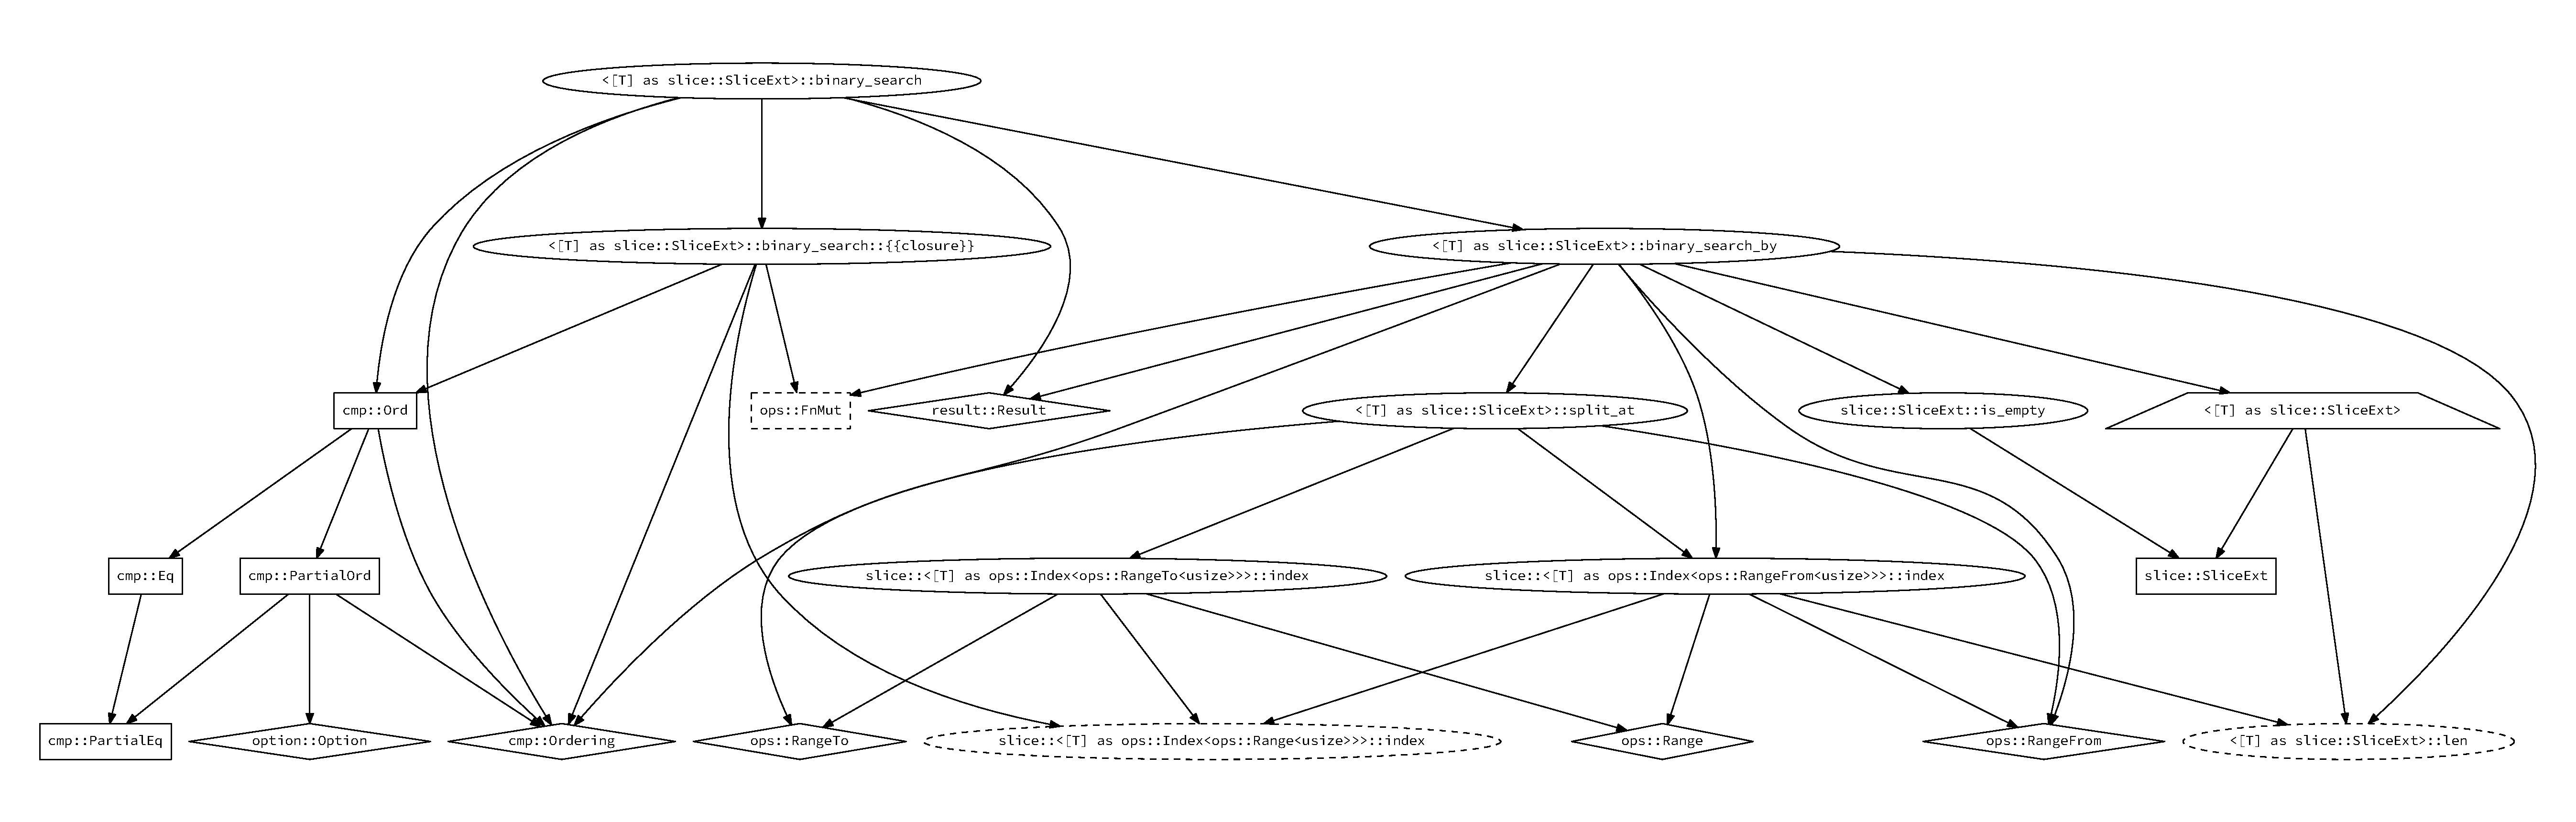
\includegraphics[width=\textwidth]{../deps}
\end{frame}

\begin{frame}[fragile]{\secname}
  \begin{minted}{rust}
fn binary_search<T>(self: &[T], x: &T) -> Result<usize, usize>
    where T: Ord
  \end{minted}
  \vfill
  \begin{minted}{lean}
definition binary_search {T : Type₁} [Ord T] (self : list T) (x : T)
  : sem (Result nat nat)
\end{minted}
\end{frame}

\begin{frame}[fragile]{\secname}
  \begin{minted}{lean}
parameter {T : Type₁}
parameter self : list T
parameter x : T
...

inductive binary_search_res : Result usize usize → Prop :=
| found     : Π i, nth self i = some x →
    binary_search_res (Result.Ok i)
| not_found : Π i, x ∉ self → sorted (insert_at self i x) →
    binary_search_res (Result.Err i)
  \end{minted} 
  \vfill  
  \begin{minted}{lean}
theorem binary_search.spec : sorted self → is_slice self →
  sem.terminates_with
    binary_search_res
    (binary_search self x) := ...
  \end{minted} 
\end{frame}

\begin{frame}[fragile]{\secname}
  \begin{minted}{lean}
definition sem (A : Type₁) := option (A × ℕ)
\end{minted}
\vfill
\begin{minted}{lean}
theorem binary_search.spec :
  ∃ f ∈ 𝓞(λ p, log₂ p.1 * p.2) [at ∞ × ∞],
  ∀ (self : list T) (x : T), is_slice self → sorted le self →
    sem.terminates_with_in
      (binary_search_res self x)
      (f (length self, Ord'.cmp_max_cost x self))
      (binary_search self x) := ...
  \end{minted} 
\end{frame}

\begin{frame}[t]{Evaluation}
  \begin{columns}[t]
    \column{0.45\textwidth}
    \textbf{2556 Zeilen Rust} \\
    \column{0.45\textwidth}
    \textbf{3199 Zeilen Lean} \\[1em]
    \begin{tabularx}{\textwidth}{lX}
      953 & Sonstige Lemmata \\
      838 & Verifikation \\
      287 & Schleifenkombinator \\
      194 & Asymptotische Analyse \\
      192 & Semantikmonade \\
      $\dots$
    \end{tabularx}
\end{columns}
\end{frame}

\begin{frame}[t]{Evaluation: Abdeckung der Sprachreferenz}
  \footnotesize{\url{kha.github.io/electrolysis}}

  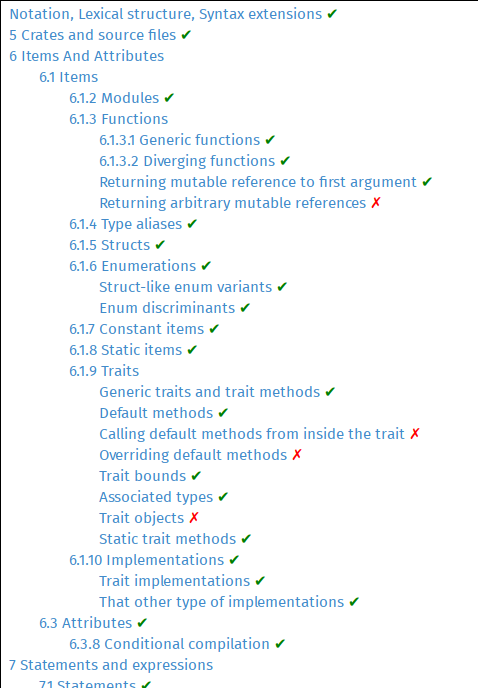
\includegraphics[height=0.9\textheight]{ref}
\end{frame}

\begin{frame}[t, fragile]{Evaluation: Abdeckung von \texttt{core}}
  \newcommand{\rowgroup}[1]{\hspace{-1em}\textbf{#1}}

  \begin{tabularx}{\textwidth}{l>{\quad}X}
    \hline
    \#definitions & \rowgroup{outcome} (reason) \\
    \hline
   6731 & \rowgroup{succeeds and type checks} \\
   2761 & \rowgroup{succeeds, but some failed dependencies} \\
   2649 & \rowgroup{translation failed} \\
    713 & overriding default method \\
    388 & \&mut nested in type \\
    360 & variadic function signature \\
    280 & float \\
    243 & raw pointer \\
    209 & cast from function pointer to usize \\
    173 & unimplemented intrinsic function \\
     45 & error from rustc API during translation \\
     40 & unimplemented rvalue  \\
     $\dots$ \\
    \hline
  \end{tabularx} 
\end{frame}

\begin{frame}[b]{Zusammenfassung}
  \begin{itemize}
    \item Das erste allgemeine Werkzeug zur Verifikation von safe Rust
    \item erfolgreich angewendet auf realen Rust-Code
    \item inklusive asymptotischer Laufzeitanalyse
    \item Breite Unterstützung der Rust-Sprache
  \end{itemize}

  \vfill

  \begin{center}
    \large\url{github.com/Kha/electrolysis}
  \end{center}

  \vfill\raggedleft\scriptsize\emph{The Rust logo is under CC-BY -- \url{https://www.rust-lang.org/en-US/legal.html}}\\
\emph{The Lean logo is under Apache-2.0 -- \url{https://github.com/leanprover/lean}}\\
\emph{Happy Ferris the Crab is under Public Domain -- \url{http://www.rustacean.net/}}\\
\end{frame}

\begin{frame}[fragile]{\texttt{Ord}-Spezifikation}
  \begin{minted}{lean}
definition ordering {T : Type₁} [decidable_linear_order T] (x y : T) :
  cmp.Ordering :=
if x < y then Ordering.Less
else if x = y then Ordering.Equal
else Ordering.Greater

structure Ord' [class] (T) extends Ord T, decidable_linear_order T :=
(cmp_eq : ∀ x y : T, Σ k, Ord.cmp x y = some (ordering x y, k))
\end{minted}
\end{frame}

\begin{frame}[fragile]{Schleifenkombinator}
  \begin{minted}{lean}
  ...

  definition terminating (s : State) :=
  ∃ Hwf : well_founded R, loop.fix s ≠ mzero

  noncomputable definition loop (s : State) : sem Res :=
  if Hex : ∃ R, terminating R s then
    @loop.fix (classical.some Hex) _ (classical.some (classical.some_spec Hex)) s
  \end{minted} 
\end{frame} 

\begin{frame}[fragile]{Schleifenkombinator}
\begin{minted}{lean}
theorem loop.terminates_with_in_ub
  {In State Res : Type₁}
  (body : In → State → sem (State + Res))
  (pre : In → State → Prop)
  (p : In → State → State → Prop)
  (q : In → State → Res → Prop)
  (citer aiter : ℕ → ℕ)
  (miter : State → ℕ)
  (cbody abody : ℕ → ℕ)
  (mbody : In → State → ℕ)
  (citer_aiter : citer ∈ 𝓞(aiter) [at ∞] ∩ Ω(1) [at ∞])
  (cbody_abody : cbody ∈ 𝓞(abody) [at ∞] ∩ Ω(1) [at ∞])
  (pre_p : ∀ args s, pre args s → p args s s)
  (step : ∀ args init s, pre args init → p args init s →
    sem.terminates_with_in (λ x, match x with
      | inl s' := p args init s' ∧ citer (miter s') < citer (miter s)
      | inr r  := q args init r
      end) (cbody (mbody args init)) (body args s)) :
  ∃ f ∈ 𝓞(λ p, aiter p.1 * abody p.2) [at ∞ × ∞], ∀ args s, pre args s →
    sem.terminates_with_in (q args s) (f (miter s, mbody args s))
      (loop (body args) s) := ...
  \end{minted}
\end{frame}
\end{document}

%%% Local Variables:
%%% mode: latex
%%% TeX-master: t
%%% End:
